\documentclass[12pt,letterpaper]{scrreprt}
\usepackage{subfigure}
\usepackage[latin1]{inputenc}
\usepackage{amsmath}
\usepackage{amsfonts}
\usepackage{amssymb}
\usepackage{graphicx}
\usepackage{todonotes}
\usepackage{appendix}
\usepackage{pdfpages}
\usepackage{lineno}
\usepackage{url}
\usepackage{enumitem}
\setlist[enumerate]{topsep=0pt,itemsep=-0.5ex,partopsep=1ex,parsep=1ex}
\setlist[itemize]{topsep=0ex,itemsep=-0.5ex,partopsep=1ex,parsep=1ex}
\usepackage[colorlinks=true,linkcolor=blue,citecolor=blue,urlcolor=blue]{hyperref}
\usepackage{mathptmx} % rm & math
\usepackage[scaled=0.90]{helvet} % ss
%\usepackage{courier} % tt
\normalfont
\usepackage[T1]{fontenc}
\addtokomafont{chapter}{\rmfamily}
\addtokomafont{section}{\rmfamily}
\addtokomafont{subsection}{\rmfamily}
\addtokomafont{subsubsection}{\rmfamily}
\addtokomafont{disposition}{\rmfamily}
\usepackage[scaled=0.9]{inconsolata}

\linenumbers

\author{P. Bachant, M. Wosnik, B. Gunawan, V. Neary}
\title{Test Plan: UNH RM2 Tow Tank Experiment}

\begin{document}

\begin{titlepage}
    \centering
    \addtolength{\topmargin}{.5in}
    {\bfseries \huge
        Experimental Test Plan---1:6 Scale Reference Model 2 Cross-Flow Turbine
    }  
    \vskip1cm
    P. Bachant$^1$\\
    M. Wosnik$^1$\\
    B. Gunawan$^2$\\
    V. Neary$^2$\\  
    \vfill
    $^1$Center for Ocean Renewable Energy \\
    University of New Hampshire \\
    Durham, NH \\
    \vspace{0.1in}
    $^2$Water Power Technologies \\
    Sandia National Laboratories \\
    Albuquerque, NM \\
    \vfill
    December 15, 2014
    \vfill
    \textbf{Prepared by:}\\
    Center for Ocean Renewable Energy\\
    University of New Hampshire\\
    Durham, NH\\
    \vspace{0.1in}
    \textbf{Prepared for:} \\
    Wind and Water Power Technologies Program \\
    Office of Energy Efficiency and Renewable Energy \\
    U.S. Department of Energy \\
    Washington, D.C.
    \vfill
    
\includegraphics[width=0.32\textwidth]{Figures/unhlogo} \\
    \vspace{0.1in}
    
\includegraphics[width=0.41\textwidth]{Figures/snllogo} \\
    \vspace{0.1in}
    
\includegraphics[width=0.34\textwidth]{Figures/doelogo}
    \vfill
\end{titlepage}

\tableofcontents

\chapter{Introduction}

Sandia National Laboratory (SNL) developed the cross-flow turbine, Reference
Model 2 (RM2), to estimate the levelized cost of energy (LCOE), and to provide
publicly available power performance data from scaled model testing that can be used to
validate open-source design tools.  More details on the reference modeling
effort are provided in Neary et al. \cite{Neary2014}.

Dimensional analysis provides scaling laws that are used to upscale model test
data into performance and design information for a full-scale prototype turbine.
For hydrokinetic turbines, hydrodynamic similitude is achieved when the Reynolds
number
\begin{equation}
Re_L = \frac{UL}{\nu},
\label{eq-Re}
\end{equation}
where $U$ and $L$ are characteristic length scales, and $\nu$ is the fluid
kinematic viscosity, Froude number
\begin{equation}
Fr = \frac{U}{\sqrt{gL}},
\label{eq-Fr}
\end{equation}
where $g$ is the gravitational acceleration, and the tip speed ratio
\begin{equation}
\lambda=\frac{\omega R}{U_\infty},
\end{equation}
where $\omega$ and $R$ are the rotor angular velocity and radius,
respectively---of the model and the full-scale device are matched. It is rare to
achieve perfect similitude for $Re$, but a threshold value should be exceeded,
such that scale model results can be extrapolated. Note that in this study we
are focusing on $Re$, not $Fr$ as the dominant scaling parameter since the
Froude number (based on blade tip submergence) will remain small (significantly below one).

As a cross-flow turbine, the RM2 blades will experience large variations in
angles of attack as they rotate about their axis (``cross-flow turbine'' means
the axis of rotation is perpendicular to flow direction---can be vertical or
horizontal). This range of angles of attack becomes larger as the tip speed
ratio decreases \cite{Para2002}. The variation is typically sufficiently large
that the blades operate under dynamic stall, which is a complex unsteady
process and deviates significantly from static foil behavior, during part of the rotation. Furthermore, the
higher the solidity of a cross-flow turbine, the lower the optimal tip-speed
ratio at which it operates. Marine Hydrokinetic (MHK) cross-flow turbines
typically have higher solidity than cross-flow wind turbines (VAWT), and hence
operate at lower tip-speed ratios. Since MHK turbines operate in a higher
density fluid, unsteady dynamic effects related to the blades' pitching motion
and flow curvature also become more important when compared to wind turbines.

The performance of cross-flow MHK turbines thus depends on both Reynolds number
and solidity (note that these issues are related, since an average blade chord
Reynolds number, $Re_{c,\mathrm{avg}} \approx \lambda U_\infty c/ \nu$, can be
expressed in terms of tip speed ratio, which is a function of solidity). If
numerical models are validated with physical model data that was obtained at
insufficiently high Reynolds numbers, it cannot be determined whether problems
with model predictions are caused by Reynolds number effects, issues related to
higher solidity, or both. It is uncertain whether numerical models validated
with physical model data obtained at low Reynolds number should be considered
validated at all, since the scale at which the model will be applied is orders
of magnitude larger. One way to overcome this uncertainty is to show that the
scaled physical model test has become Reynolds number independent, and therefore
validation efforts should be relevant at full-scale. 

For example, the effect of Reynolds number on average power output was shown to
be significant on the 2 m Sandia Research Darrieus turbine in wind tunnel
testing \cite{Blackwell1976}: Maximum power coefficient, $C_{P,\mathrm{max}}$,
increased with Reynolds number, $Re_c$, along with a shift of the location of
$C_{P,\mathrm{max}}$ toward lower tip speed ratios due to delayed blade stall.
The effects of Reynolds number were quite dramatic over a relatively small range
of $Re_c \approx 1.1 \times 10^5$--$2.9 \times 10^5$. More recently, Bachant and
Wosnik \cite{Bachant2014} showed that turbine performance and near-wake
characteristics become Reynolds number independent at $Re_c \approx 2 \times
10^5$.

The need for experimental data that is relevant to full-scale behavior stems
from the need to validate numerical models---most importantly mid-fidelity
models---desirable for MHK developers to predict the performance of their
cross-flow turbine designs, since physical modeling at appropriate scales can be
prohibitively expensive in the early stages of engineering. Furthermore,
Navier--Stokes-based computational fluid dynamics (CFD) simulations require
modeling in 3 dimensions, which generally necessitates high performance
computing---a resource that is not commonly available, and more expensive.

To date, attempts to validate SNL's mid-fidelity CACTUS vortex line model
\cite{Murray2011} have relied on measurements from the Saint Anthony Falls
Laboratory (SAFL) \cite{Hill2014} and the University of New Hampshire (UNH)
\cite{Neary2013, Michelen2014}. For the SAFL experiments (RM2), the chord
Reynolds number, $Re_c \sim 10^4$, was below the threshold needed to properly
simulate lift and stall characteristics. For the UNH experiment
\cite{Bachant2013}, the chord Reynolds number was sufficiently high at $Re_c
\approx 2.7 \times 10^5$, but the chord/radius ratio and solidity (13.4\%)
created instability in the free-wake evolution in the model, which caused significant
overestimation of power coefficient.

The present task is to acquire a new dataset for the lower solidity
RM2 turbine, but at higher Reynolds numbers than those achieved in the experiments at SAFL. It is also suspected that the strut
drag model in CACTUS could be the source of some discrepancy, so the strut drag will be deliberately modified in the physical model to provide data to help sort out that question. This dataset will be
publicly available for both validation of CACTUS and other numerical models.
This report details the experimental test plan for acquiring, processing, and
archiving this data, which includes development of a scaled physical model, and
descriptions of the experimental setup and procedure to be performed in a towing
tank at the University of New Hampshire (UNH).


\section{Study goals and objectives}

The overarching goal of this project is to collect a Reynolds number independent
performance dataset for a 1:6 scale RM2 turbine, which is repeatable, and which
can be used to investigate the accuracy of numerical models, e.g., mid-fidelity
models such as CACTUS. The project will provide insight on the physics of
hydrokinetic cross-flow turbines, including the importance of blade strut drag
on turbine power output, which will determine what level of focus is necessary
in improving mid-fidelity modeling of these effects, and also give turbine
designers some perspective on the need to mitigate strut drag to improve rotor
efficiency. The experimental dataset will be shared publicly and can be used for
validating other numerical models/codes used by developers and DOE partners. The
study goals can be distilled into the following main objectives:

\begin{itemize}
	\item Design and fabricate a 1:6 scale model of the RM2 turbine.

	\item Perform measurements with the RM2 1:6 scale model in the UNH-CORE tow
	tank turbine test bed to:

	\begin{itemize}
		\item Document the dependence of the turbine power coefficient on Reynolds
		number, and where it becomes independent of Reynolds number.
		
		\item Characterize the near-wake at maximum power coefficient at the Reynolds
		number independent state.
		
		\item Observe the influence of strut drag on turbine performance.
	\end{itemize}

	\item Write a technical report to document the study objectives, methods,
	results, and conclusions.
	
	\item Analyze and archive measurements as an open model validation dataset.
\end{itemize}

\chapter{Experimental setup and methods}

Turbine performance is characterized by the nondimensional power coefficient
\begin{equation}
C_P = \frac{P}{\frac{1}{2} \rho A U_\infty^3},
\label{eq-cp}
\end{equation}
where $P$ is the mechanical power output (the product of the shaft torque $T$
and angular velocity $\omega$), $\rho$ is the fluid density, $A$ is the
turbine's frontal area, and $U_\infty$ is the free stream velocity. Also of
interest is the overall drag (a.k.a. thrust) coefficient the device imparts on
the flow in which its placed, defined as
\begin{equation}
C_D = \frac{F_D}{\frac{1}{2} \rho A U_\infty^2},
\label{eq-cd}
\end{equation}
where $F_D$ is the streamwise component of the force on the rotor.

A performance curve, which is a plot of $C_P$ versus nondimensional rotation
rate---tip speed ratio $\lambda$---describes the device's behavior over its
range of operation. An example of is shown in Figure~\ref{fig-cp}. In this
experiment we will create similar curves by measuring turbine power coefficient
over a range of prescribed $\lambda$, where the tow speed, or turbine diameter
Reynolds number $Re_D$ is held constant. By creating curves for various $Re_D$,
we seek a condition where the power coefficient at the optimal tip speed ratio
begins to converge asymptotically to some limit, similar to the approach used in
\cite{Bachant2014}, the data from which is plotted in
Figure~\ref{fig-cp_re_dep}.

\begin{figure}[ht]
\centering
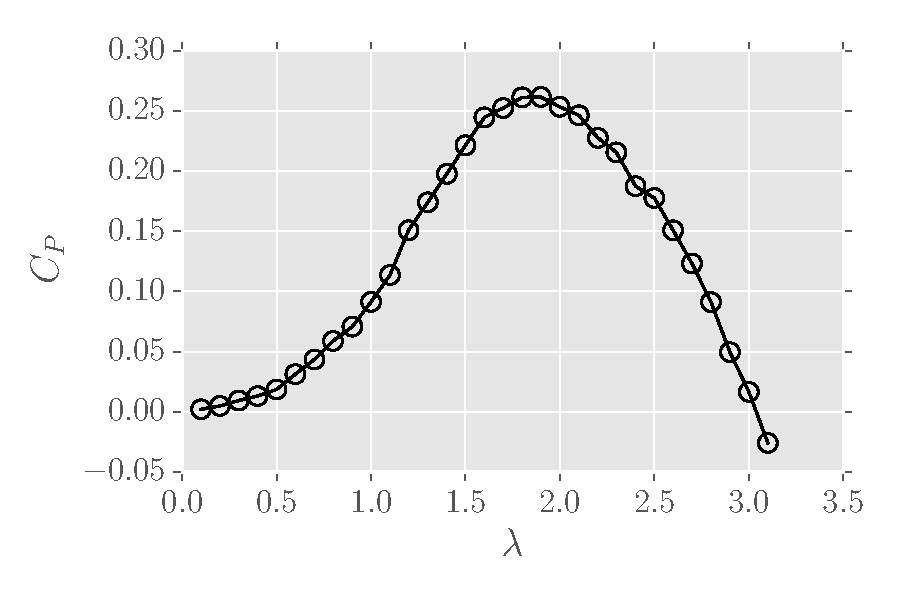
\includegraphics[width=0.65\textwidth]{Figures/cp_vs_tsr.pdf}
\caption{Example of a turbine performance curve.}
\label{fig-cp}
\end{figure}

\begin{figure}[ht]
\centering
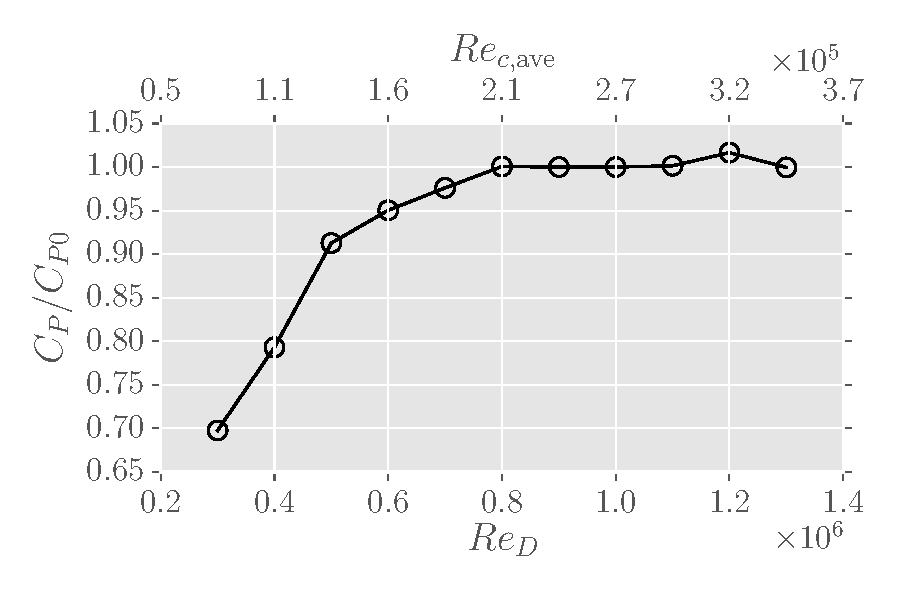
\includegraphics[width=0.65\textwidth]{Figures/re_dep_cp.pdf}
\caption{Normalized turbine power coefficient plotted versus Reynolds number, adapted from \cite{Bachant2014}.}
\label{fig-cp_re_dep}
\end{figure}

\section{Facility and instrumentation}

Experiments will be performed in the UNH tow/wave tank, a 36 m long facility
with a 3.66 m wide by 2.44 m deep cross-section, capable of tow speeds up to 3
m/s\footnote{Note that though 3 m/s is the technical limit, the practical limit
for achieving substantial tow durations is approximately 2 m/s.}, pictured in
Figure~\ref{fig-tow_tank}. The turbine will be mounted in a frame built from
NACA 0020 struts, attached to the tow carriage by four linear bearings, which
transfer all streamwise force to a pair of S-beam load cells. The turbine shaft
RPM will be controlled by a servo motor system, which allows prescription of the
turbine tip speed ratio. The load torque will be measured by an inline rotary
torque transducer and a load cell mounted at a fixed distance from the servo
motor, providing a redundant measurement. Turbine shaft angle will be measured
using the servo drive's emulated encoder output, set to $10^5$ counts per
turbine shaft revolution. Carriage speed, and therefore inflow velocity will be
measured using a linear encoder with 10 $\mu$m resolution. All of these
performance-related quantities will be sampled as 2 kHz, while the tow tank's
motion controller will provide redundant measurements of the carriage speed and
turbine angular velocity sampled at 1 kHz. Turbine wake measurements at 1
turbine diameter downstream will be measured with a Nortek Vectrino+ acoustic
Doppler velocimeter, sampling at 200 Hz. A list of the sensors to be used in the
experiment is shown in Table~\ref{tab-sensors}, instrumentation in
Table~\ref{tab-instrumentation}, and a drawing of the experimental setup is
shown in Figure~\ref{fig-exp_setup}.


\begin{figure}[ht!]
\centering 
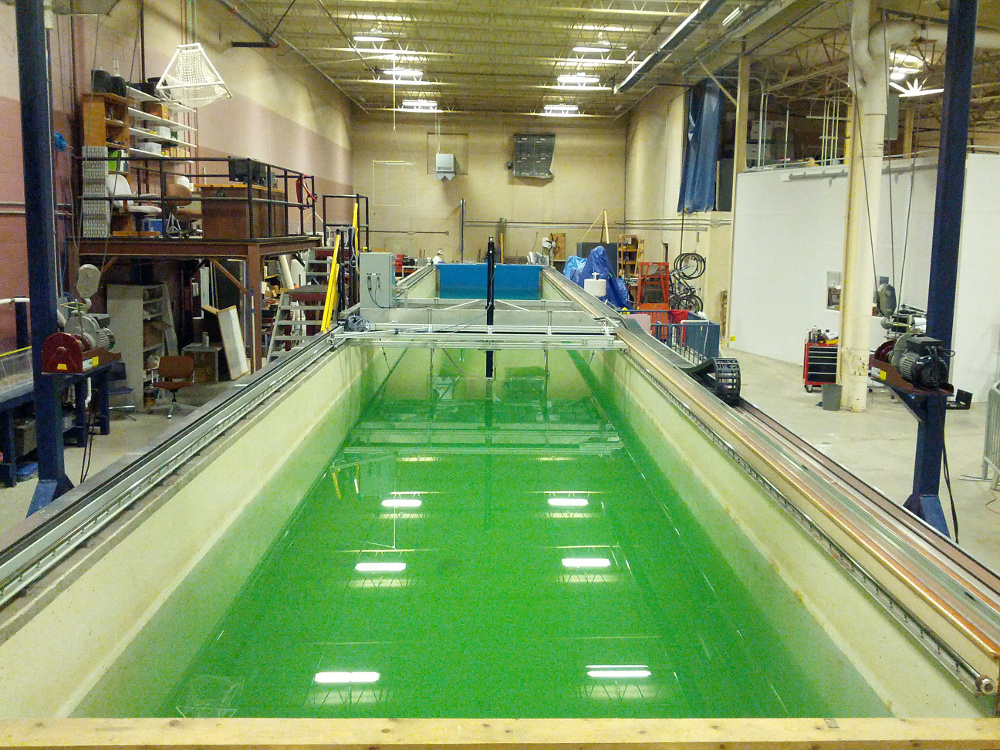
\includegraphics[clip,trim=0 0.4in 0 0.37in, 
width=0.49\textwidth]{Figures/tow_tank_length} 
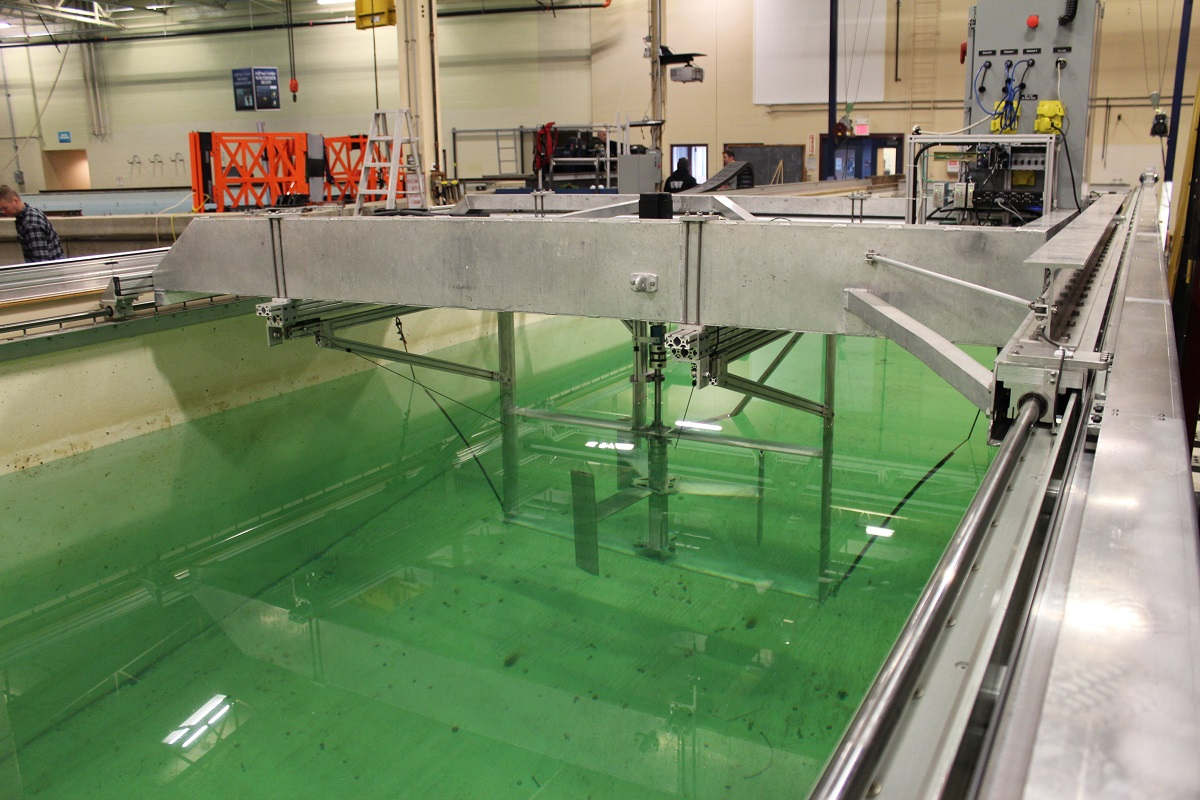
\includegraphics[clip,trim=0.67in 0 0 0, 
width=0.49\textwidth]{Figures/test_bed_photo} 
\caption{Photos of the UNH towing tank and turbine test bed.} 
\label{fig-tow_tank}
\end{figure}


\begin{table}[ht]
\centering
\begin{tabular}{c|c|c|c}
Measured quantity & Device type & Mfg. \& model & Nominal accuracy \\
\hline 
Carriage position & Linear encoder & Renishaw LM15 & 10 $\mu$m/pulse \cite{RenishawLM15}\\
Turbine angle & Servo encoder output & Kollmorgen AKD & 10$^5$ pulse/rev \cite{KollmorgenAKD}\\
Turbine torque & Rotary transducer & Interface T8-200 & $\pm$0.5 Nm \cite{InterfaceT8}\\ 
Turbine torque (2) & Load cell (\& arm) & Sentran ZB3-200 & $\pm$0.2 Nm \cite{SentranZB}\\
Drag force, left & Load cell & Sentran ZB3-500 & $\pm$0.6 N \cite{SentranZB}\\
Drag force, right & Load cell & Sentran ZB3-500 & $\pm$0.6 N \cite{SentranZB}\\
Fluid velocity & ADV & Nortek Vectrino+ & $\pm$0.5\% $\pm$1 mm/s \cite{NortekVectrino}\\
\end{tabular}
\caption{Details of the sensors to be used for the experiment. Note that ``(2)''
denotes a secondary redundant measurement. ``Turbine torque (2)'' nominal
accuracy estimated by combining load cell accuracy and arm machining tolerances
($\pm 1 \times 10^{-4}$ m) as root-sum-square.} \label{tab-sensors}
\end{table}

\begin{table}[ht]
\centering
\begin{tabular}{c|c|c}
Measured quantity & Device type & Mfg. \& model \\
\hline 
Carriage position & Differential counter & NI 9411 \\
Carriage velocity (2) & Motion controller & ACS NTM \\
Turbine angle & Differential counter & NI 9411 \\
Turbine RPM (2) & Motion controller & ACS NTM \\
Turbine torque & Analog voltage input & NI 9405 \\ 
Turbine torque (2) & Analog bridge input & NI 9237 \\
Drag force, left & Analog bridge input & NI 9237 \\
Drag force, right & Analog bridge input & NI 9237 \\
\end{tabular}
\caption{Details of the instrumentation to be used for the experiment. Note that
``(2)'' denotes a secondary redundant measurement.}
\label{tab-instrumentation}
\end{table}

\begin{figure}[ht]
\centering
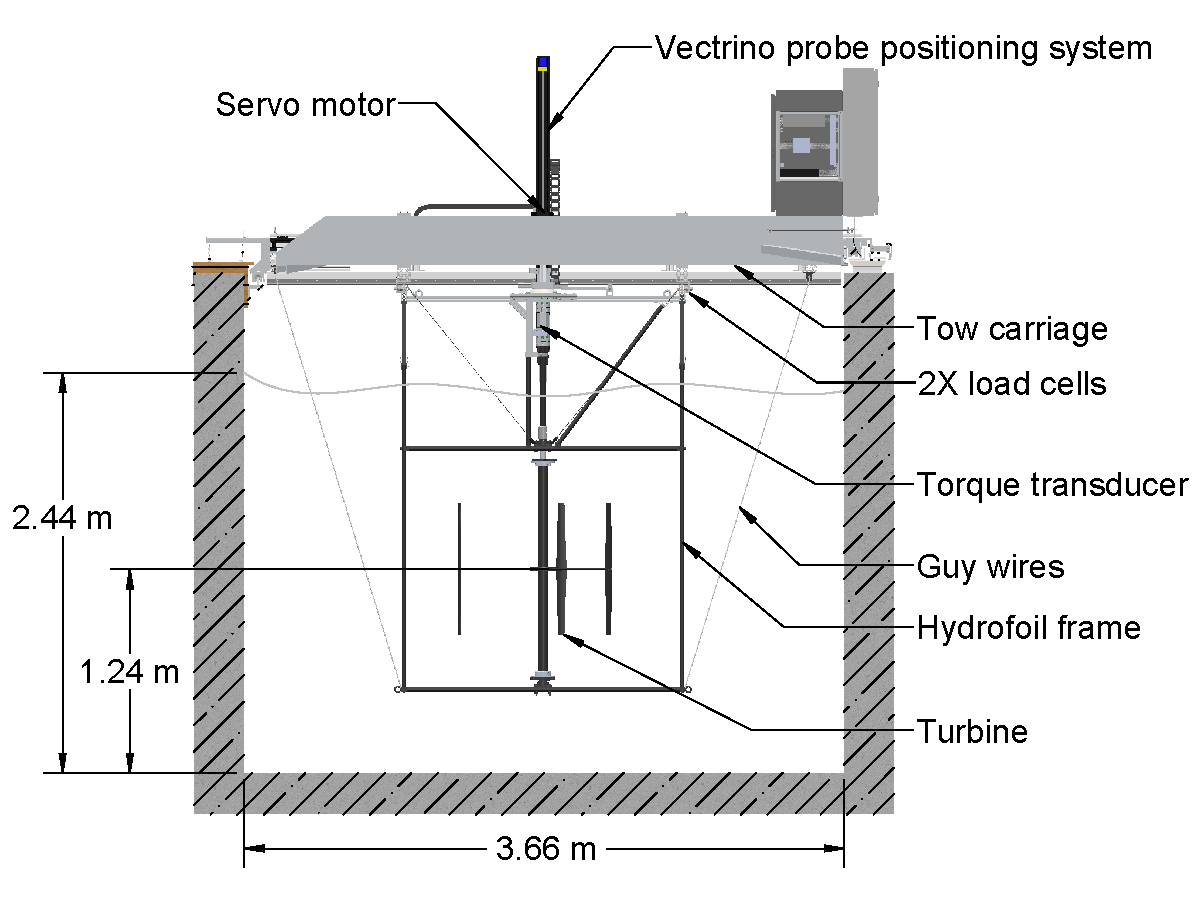
\includegraphics[clip,trim=0.01in 0 0 0, width=0.95\textwidth]{Figures/tank_cross_section}
\caption{Illustration of the experimental setup.}
\label{fig-exp_setup}
\end{figure}


\subsection{Calibrations}

Before collecting data, traceable calibration certificates will be obtained for
the Interface T8-200 torque transducer and NI 9405 and NI 9237 modules. The
torque transducer calibration will be used directly in data processing, while
the load cells will be calibrated using an additional Sentran ZB S-beam load
cell and indicator, a package which will also have its own calibration
certificate. The redundant torque measurement load cell/arm system will also be
calibrated using the Sentran load cell and indicator, attached to a fixture with
a distance from the axis of rotation known to within approximately 0.005 inches.

\subsection{Synchronization of instrumentation subsystems}

The three data acquisition instrumentation subsystems---motion controller, NI
DAQ (performance measurements), and Vectrino+ (wake velocity
measurements)---will begin sampling at precisely the same time each run, after
being triggered by a TTL pulse created by the motion controller. This strategy
retains synchronization for all performance signal samples (tow speed, torque,
drag, angular velocity), ensuring precise calculation of, e.g., power
coefficient. Since there is also synchronization of the initial sample from each
three subsystems, correlation of events in the performance and wake signals is
also possible.

\subsection{Tare drag and torque compensation} 

Tare torque and drag runs will also be performed to measure the shaft bearing
friction torque and turbine mounting frame drag, respectively. These data will
be similar to the turbine performance data, omitting torque measurements for the
tare drag runs and vice versa. Tare drag runs will be performed for each tow
speed in the experiment, for which the mean value is used in data processing.
Tare torque runs will be performed by rotating the turbine shaft (without
blades) in air at constant angular velocity for a specified duration, over the
range of angular velocities used throughout the experiment. Tare torque will
then be fit with a linear regression versus shaft angular velocity, and added to
the measured turbine torque in post-processing.

\section{Turbine model}

The turbine is to be a 1:6 scale model of the RM2 rotor, reproduced as
faithfully as possible. Turbine geometry is to be scaled from the RM2 ``rev 0''
design report \cite{Barone2011}, with the exception of the shaft diameter, which
will be a scaled version of the SAFL RM2 shaft \cite{Hill2014}. The hub design
is also similar to the SAFL model, which may aid in comparison of the results,
though this is not a top priority. Geometric parameters are shown in
Table~\ref{tab-turb_geom} and a drawing of the turbine design is shown in
Figure~\ref{fig-turbine_drawing}. The turbine model components---blades, struts,
shaft, and center hub sections---will be fabricated from 6061-T6 aluminum, which
will be hardcoat anodized per MIL-8625-A, type III, class 2 specifications.

\begin{table}[ht]
\centering
\begin{tabular}{l|l|l}
   & Full-scale & Model (1:6) \\
\hline 
Diameter (m)   & 6.450 & 1.075 \\ 
Height (m)     & 4.840 & 0.8067 \\ 
Blade root chord (m) & 0.4000 & 0.06667 \\ 
Blade tip chord (m)  & 0.2400 & 0.04000 \\ 
Blade profile & NACA 0021 & NACA 0021 \\ 
Blade mount & 1/2 chord & 1/2 chord \\ 
Blade pitch (deg.) & 0.0 & 0.0 \\ 
Strut profile & NACA 0021 & NACA 0021 \\ 
Strut chord (m) & 0.3600 & 0.06000 \\ 
Shaft diameter (m) & 0.2540 \cite{Beam2011} or 0.4160 \cite{Hill2014} & 0.06350\\ 
\end{tabular}
\caption{RM2 turbine geometric parameters.}
\label{tab-turb_geom}
\end{table}

\begin{figure}[ht]
\centering
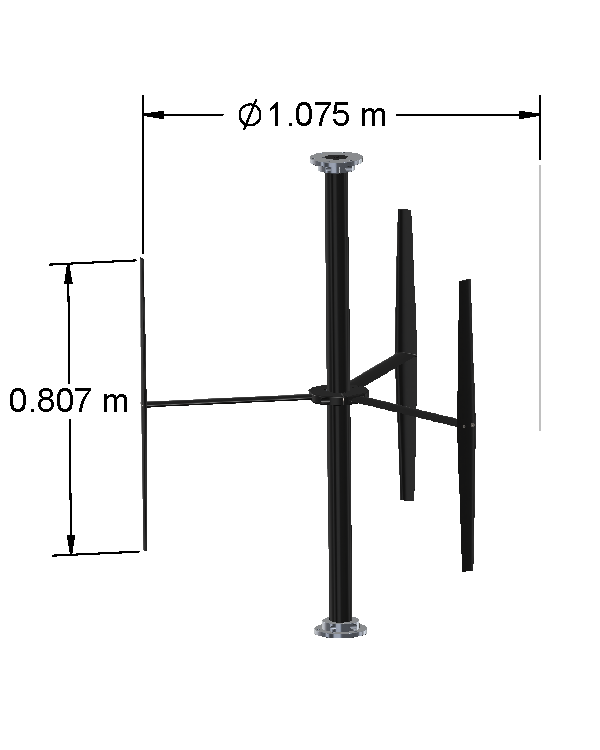
\includegraphics[width=0.5\textwidth]{Figures/turbine}
\caption{Illustration of the UNH RM2 scaled physical model.}
\label{fig-turbine_drawing}
\end{figure}


\section{Test parameters}

Data collection runs will take place during individual tows, for which all
independent variables---tow speed, tip speed ratio, velocity probe
position---are held constant. These runs can then be grouped into logical test
matrix ``sections,'' in which typically a single independent variable is varied.
For example, a test matrix section will be dedicated to collecting turbine
performance curves for a single tow speed, or turbine diameter Reynolds number,
where only tip speed ratio is varied. Note that the upper limit of tip speed
ratio will be determined in ``shakedown'' runs, and chosen to be just above the
value at which turbine power coefficient reaches zero. Additional performance
curve test matrix sections will be created/executed for different tow speeds.
For wake characterization, test matrix sections will vary the cross-stream
position of the velocity probe, providing a single profile transverse, and
multiple profiles will be taken at varying vertical locations. Examples of test
matrices for a performance curve and a wake profile are shown in
Table~\ref{tab-test_section}.

Parameters for each test matrix section will be created in the
\texttt{Config/Test plan} folder inside the experiment working directory, saved
in comma separated value (CSV) format as input to the
\textit{TurbineDAQ}\footnote{\url{https://github.com/petebachant/TurbineDAQ}}
experiment automation software, which was developed specifically for
vertical-axis turbine measurements in the UNH tow tank (see
Figure~\ref{fig-turbinedaq} for a screenshot). These CSVs also provide
information about each run to be used in post-processing. Note that the software
is designed to read turbine properties (from
\texttt{Config/turbine\_properties.json}), e.g. radius and height, so inputs for
turbine rotational speed (tip speed ratio) and Vectrino probe location are in
nondimensional form.


\section{Determining tank settling time}

Sample tows will be done to determine the amount of time taken between runs such
that the tank has settled adequately, i.e., background turbulence and any large
scale mean flows have been dissipated. The settling times will be stored in the
experiment configuration---one value for each tow speed.


\section{Determining Reynolds number independence}

In order to establish that we have reached a Reynolds number independent regime
for turbine performance, we will acquire multiple performance curves, starting
at a relatively slow tow speed (on the order of 0.2 m/s), incrementing up to the
maximum practical tow speed. For the scale of the RM2 model, we expect to see
convergence in the measured power coefficient, similar to
Figure~\ref{fig-cp_re_dep}, around a tow speed of 1 m/s, which corresponds to a
turbine diameter Reynolds number $Re_D = 1.1 \times 10^6$ and an approximate
blade chord Reynolds number $Re_c = 2.0 \times 10^5$ at $\lambda = 3$. This will
be determined by post-processing the data concurrently. See Table~\ref{tab-re}
for Reynolds numbers corresponding to specific tow speeds.

\begin{table}[ht]
\centering
\begin{tabular}{c|c|c}
Tow speed (m/s) & $Re_D$ & $Re_c$ at $\lambda = 3$ \\ 
\hline 
0.2 & $2.2 \times 10^5$ & $4.0 \times 10^4$ \\ 
0.4 & $4.3 \times 10^5$ & $8.0 \times 10^4$ \\ 
0.6 & $6.5 \times 10^5$ & $1.2 \times 10^5$ \\ 
0.8 & $8.6 \times 10^5$ & $1.6 \times 10^5$ \\ 
1.0 & $1.1 \times 10^6$ & $2.0 \times 10^5$ \\ 
1.2 & $1.3 \times 10^6$ & $2.4 \times 10^5$ \\ 
1.4 & $1.5 \times 10^6$ & $2.8 \times 10^5$ \\
\end{tabular} 
\caption{Turbine diameter and approximate blade chord Reynolds numbers
corresponding to tow speeds.} \label{tab-re}
\end{table}


\section{Measuring the effects of strut drag}

In order to measure the effects of strut drag, we will acquire an additional
performance curve at the Reynolds number independent tow speed $U_0$ for the
device with cylindrical strut covers slid over the struts to increase their drag
by several orders of magnitude. We will also measure the rotor
torque with the blades removed and strut covers installed, while rotating the
turbine over the range of angular velocities seen in the performance curve,
providing a comparison for the drag coefficient of the cylinders in a rotating
flow. An illustraction of the turbine with strut covers installed---both with
and without blades---is shown in Figure~\ref{fig-strut_covers}.

\begin{figure}[!ht]
\centering
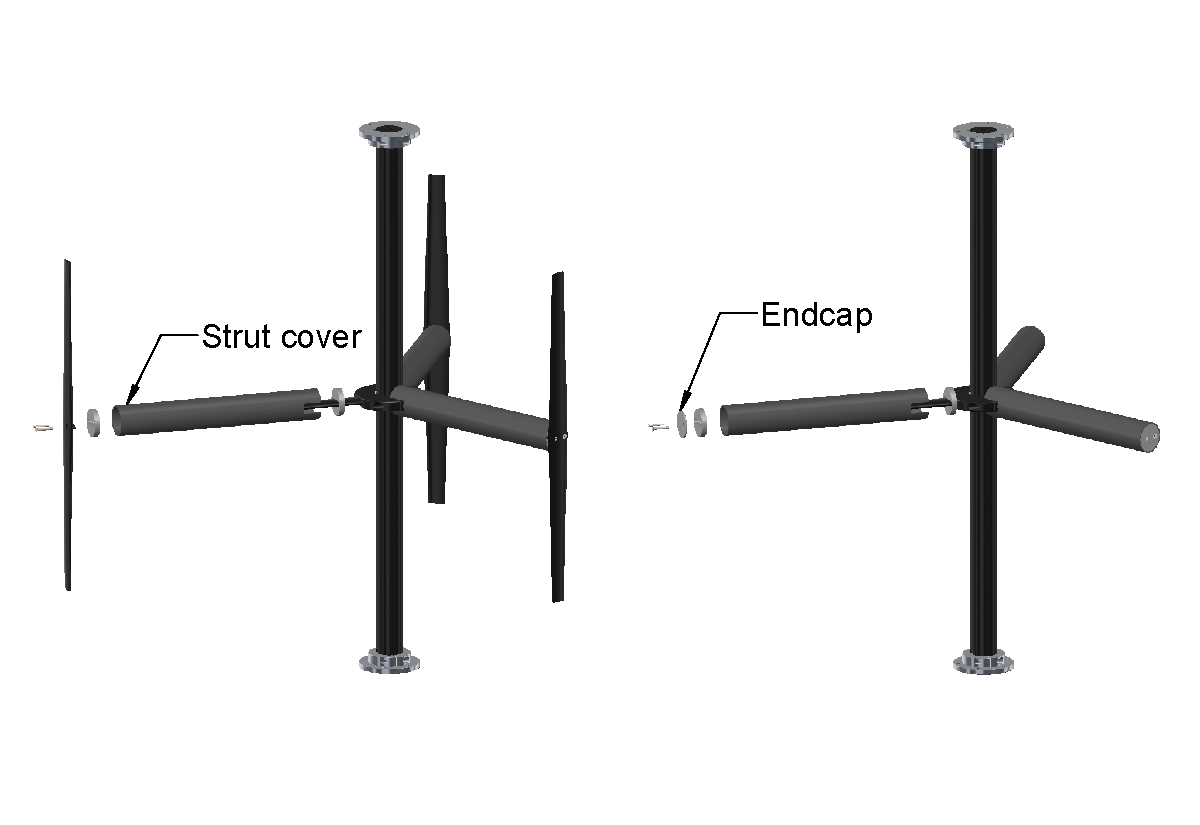
\includegraphics[width=0.8\textwidth]{Figures/strut_covers}
\caption{Illustration of strut cover design with (left) and without (right)
blades installed.}
\label{fig-strut_covers}
\end{figure}

\section{Near-wake characterization}

After Reynolds number independence has been found, we will perform a
characterization of the near-wake at one turbine diameter downstream, acquiring
a series of cross-stream profiles at varying height, mapping out the upper half
of the wake, measured from the turbine center. The Vectrino will be in a fixed
location (relative to the turbine center) for each run, necessitating multiple
runs at varying cross-stream and vertical coordinates with the approximate
ranges $y/R = \pm 2.8$ and $z/H = 0$--$0.75$, respectively---chosen based on
previous experiments with similarly sized turbines, e.g. \cite{Bachant2013}, to
visualize the complex three-dimensional flow field present in the near-wake. The
probe will be mounted to a NACA 0020 strut, attached to an automated positioning
system, shown in Figure~\ref{fig-yz_traverse}, which is driven by stepper motors
with resolutions of approximately $3 \times 10^{-5}$ meters per step, and
controlled by the tow tank's main motion controller.

\begin{figure}[ht]
\centering
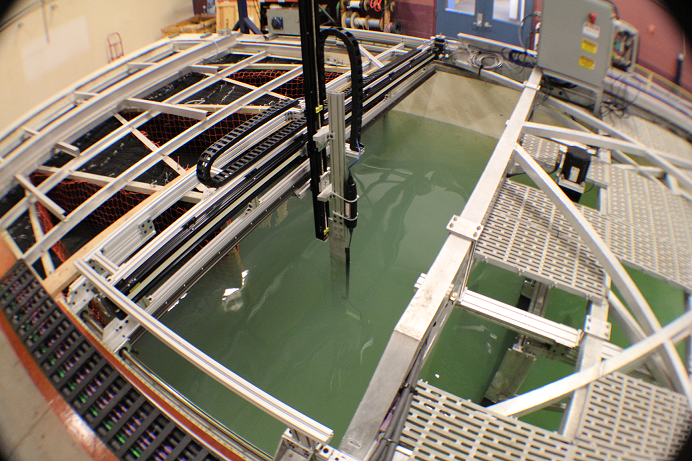
\includegraphics[width=0.6\textwidth]{Figures/yz_traverse}
\caption{Photograph of the Vectrino probe positioning system.}
\label{fig-yz_traverse}
\end{figure}

\section{Data processing}

Turbine shaft angular velocity and carriage speed must be computed by taking the
derivatives of the measured position time series. This will be done using a
second order central difference scheme, and may be subsequently filtered with a
moving average filter to help reduce noise introduced by the differentiation. To
check that excess high frequency energy was not removed during filtering, the
velocity signals can be compared to their redundant measurements recorded from
the motion controller.

After the velocity time series are calculated, they are used to calculate time
series for instantaneous $\lambda$, $C_P$, and $C_D$, from which mean values are
computed.

Data collected for each run will include a transient period, where the tow
carriage accelerates, after which turbine torque and wake velocities settle to
become stationary or periodic. It is this ``steady-state'' duration that we are
interested in. The duration will be identified for several runs at each tow
speed by manual inspection. The tail end will then be truncated such that the
data to be processed includes an integer number of blade passages, to minimize
bias from periodicity. The time interval will be recorded as part of the reduced
data for each run, along with the number of blade passages and revolutions.

Wake velocity data will be post-processed using methods outlined in Gunawan et
al. \cite{Gunawan2011}. Corrections will include, for example, eliminating
and/or replacing spikes \cite{Goring2002}, Doppler noise \cite{Voulgaris1998},
and filtering \cite{Garcia2005}.

A CSV table of derived data will be created for each section, with one row per
run containing the mean and standard deviation for the run's measured tow speed,
tip speed ratio, power coefficient, drag coefficient, $u$, $v$, and $w$
components of wake velocity, along with $\overline{u'v'}$, $\overline{u'w'}$,
and $\overline{v'w'}$ Reynolds stresses, turbulence kinetic energy $k$, and 95\%
confidence expanded uncertainties for $\lambda$, $C_P$, and $C_D$ (see
\ref{heading-uncertainty} for the uncertainty analysis procedure). These CSV
files will be stored in the \texttt{Data/Processed} directory, which will be
included in the experiment's version control repository, to track changes to
derived data from, e.g., modifications to the processing code.

\subsection{Uncertainty analysis}\label{heading-uncertainty}

As mentioned previously, one of the primary uses for the data collected is
comparison with results from numerical modeling, and this comparison requires an
estimate for what range of values from the experimental result includes the true
value. This range---or uncertainty---results from a combination of systematic
and random errors. The random error can be inferred from the sample standard
deviation and the systematic from the sensor calibrations or datasheets.
Combining both sources of error, along with their propagation into quantities
derived from multiple measurements, will follow the procedures outlined in
Coleman and Steele (2009) \cite{ColemanSteele}, described below.

An expanded uncertainty interval with 95\% confidence can be computed for
$\lambda$, $C_P$, and $C_D$
\begin{equation}
U_{95} = t_{95} u_c,
\end{equation}
where $t_{95}$ is the value from the Student-$t$ distribution for a 95\%
confidence interval and $u_c$ is the combined standard uncertainty. Combined
standard uncertainty for a given quantity $X$ is calculated by
\begin{equation}
u_X^2 = s_X^2 + b_X^2,
\end{equation}
where $s_X$ is the sample standard deviation, calculated as the standard
deviation of the mean per turbine revolution, and $b_X$ is the systematic
uncertainty, computed by
\begin{equation}
b_{X}^2 = \sum_{i=1}^J \left( \frac{\partial X}{\partial x_i} \right)^2 b_{x_i}^2,
\end{equation}
where $x_i$ is a primitive quantity used to calculate $X$ (e.g. $T$, $\omega$,
and $U_\infty$ for calculating $C_P$), and $b_{x_i}$ is the primitive quantity's
systematic uncertainty, estimated as half the value listed in
Table~\ref{tab-sensors}.

Selecting $t_{95}$ requires an estimate for degrees of freedom $\nu_X$, which can
be obtained using the Welch--Satterthwaite formula
\begin{equation}
\nu_X = \frac{\left(s_X^2 + \sum_{k=1}^M b_k^2 \right)^2}
             {s_X^4/\nu_{s_X} + \sum_{k=1}^M b_k^4/\nu_{b_k}},
\end{equation}
where $\nu_{s_X}$ is the number of degrees of freedom associated with $s_X$ and
$\nu_{b_k}$ is the number of degrees of freedom associated with $b_k$.
$\nu_{s_X}$ is assumed to be $(N-1)$, where $N$ is the number of independent
samples (or turbine revolutions). $\nu_{b_k}$ will be estimated as
\begin{equation}
\nu_{b_k} = \frac{1}{2} \left( \frac{\Delta b_k}{b_k} \right)^{-2},
\end{equation}
where the quantity in parentheses is the relative uncertainty of $b_k$.

From previous measurements of a similarly-sized vertical-axis turbine with the
same experimental setup, we expect expanded uncertainties for $\lambda$, $C_P$,
and $C_D$ to be approximately 0.008, 0.01, and 0.02, respectively, at a tow
speed $U_\infty = 1.0$ m/s. These values are well within the discrepancies
between previous measurements and predictions by CACTUS \cite{Michelen2014},
making the data from the experiments described here suitable for model validation.

\chapter{Research deliverables}

The research deliverables for this project include the following:

\begin{itemize}

    \item A 1:6 scale RM2 vertical-axis turbine rotor model, 3-D CAD models of
    its geometry, and 2-D manufacturing drawings detailing how it was fabricated
    and assembled.
    
    \item Raw turbine performance data for power coefficient curves acquired at
    multiple Reynolds numbers. The data are described in detail in
    Section~\ref{sec-exp_data} below.
    
    \item Raw turbine performance data showing the parasitic effects of
    high-drag support struts.
    
    \item Three components of raw wake velocity data characterizing the upper
    half of the wake a one turbine diameter downstream.
    
    \item Tabulated processed data from each run and the software used to
    compute them.
    
    \item A final report detailing the goals of the experiment, how it was
    conducted, descriptions of the results, and conclusions reached.

\end{itemize}


\section{Experimental data}\label{sec-exp_data}

Each data collection run (one tow) will produce raw data for the turbine torque,
drag force on the submerged equipment, turbine shaft angle, carriage position,
and Vectrino velocity measurements, along with the relative times for the
samples. Raw data will be stored in HDF5 format, additional Vectrino raw data in
Nortek's binary format (\texttt{*.vno}), run metadata in text-based JavaScript
Object Notation (JSON), processed data as CSV, and processing code in Python.
These formats were chosen for their platform- and language-independence, which
will allow broadest usage of the data by other researchers. A summary of data
file types, names, and contents is presented in
Table~\ref{tab-data_description}.

\subsection{Directory structure and naming conventions}

A sample directory structure is shown in Figure~\ref{fig-dir_structure}. In the
\texttt{Config/Test plan} folder are the CSV files containing the tabulated test
parameters for each test matrix section, whose names are inferred from the CSV
file names. Raw data files are stored in the
\texttt{Data/Raw/\{section\}/\{run\}} subfolders, while processed data are
stored in the \texttt{Data/Processed} subfolder---one CSV file per test matrix
section.

\subsection{Metadata}

Each run's metadata file (\texttt{metadata.json}) will include:

\begin{itemize}

	\item Nominal tow speed
	
	\item Prescribed tip speed ratio
	
	\item Test matrix section and run number, e.g., ``\texttt{Perf-0.8 run 4}''
	
	\item Time created
	
	\item Turbine name, radius, and height
	
	\item \textit{TurbineDAQ} software version
	
	\item Vectrino location
	
	\item Vectrino metadata (Note: Additional Vectrino metadata will be included in
	the \texttt{*.vno} files.):
	
		\begin{itemize}
		
			\item Coordinate system
			
			\item Sample rate
			
			\item Velocity range index
		
		\end{itemize}
		
	\item NI DAQ device channel metadata:
	
		\begin{itemize}
		
		\item Sample rate
		
		\item Scale names, slopes, $y$-intercepts, and units 
		
		\end{itemize}

\end{itemize}


\section{Management and archiving}

This experiment will likely produce on the order of 10 GB of data. The two
guiding principles for the management of this data are openness and usefulness,
i.e., we want potential users to know exactly how the data was created, and be
able to reuse the data as conveniently as possible. We will make available all
raw and processed data, along with any software written for the processing,
analysis, and visualization of this data. It is also important that we provide
the data and code such that they are maintainable, both by ourselves and by
other users.

Since the dataset is of moderate size, we will split the data into two
parts---one containing the processed data, and one the raw data. This will allow
users to first obtain the processed data, processing code, and
documentation---most relevant for generating figures or comparing to numerical
modeling results---without having to download an excessively large archive.
However, if users want to reanalyze the raw data, the processing code will be
written such that raw data files are downloaded as needed, rather than one bulk
download, though it will still be possible to download the entire raw dataset,
if desired. This strategy is convenient, for example, for a researcher looking
to compute wake spectra at a single location, since he or she would only need to
download $\sim 10$ MB of data, rather than the entire $\sim 10$ GB.

Raw data files will be uploaded to figshare\footnote{\url{http://figshare.com}},
which will then give the dataset a Digital Object Identifier (DOI) and therefore
a persistent URL. Processed data, processing code, and documentation will be
stored in a Git\footnote{\url{http://git-scm.com}} version control repository,
hosted on GitHub\footnote{\url{https://github.com/UNH-CORE/RM2-tow-tank}} to
help facilitate updates to the analysis by both the investigators and third
parties. Tagged versions or ``releases'' of the Git repository will be uploaded
to figshare such that they will have their own DOIs, and can be cited
appropriately in publications.

\section{Licensing} 

The research products described above---documentation, data, code, CAD models,
etc.---will be freely available under a Creative Commons Attribution (CC-BY)
license, which allows free access, further sharing, and adaptation so long as
the original source is credited.


\chapter{Summary}

In this study we will set out to acquire a Reynolds number independent dataset
for the RM2 cross-flow turbine, producing an extensive collection of raw data,
along with open repository of processed data, code, and documentation to support
numerical model validation efforts. This objective requires that we design and
build a turbine model at a scale that is expected to reach Reynolds number
independence within the UNH tow tank's tow speed range. We will then acquire
full device performance curves (power and drag coefficients) at multiple tow
speeds---or turbine diameter Reynolds numbers $Re_D = U_\infty D/ \nu$---to
attempt to find convergence. Once convergence is found, we will acquire
measurements to characterize the three-dimensional nature of the near-wake (one
turbine diameter downstream) at a threshold Reynolds number $Re_0$ using
acoustic Doppler velocimetry. Lastly, we will observe the effects of strut drag
on turbine model performance---measuring the parasitic torque from support
struts by rotating the turbine in still water, both with and without cylindrical
tubes slid over the struts to significantly increase their drag coefficients. We
will then acquire a performance curve at $Re_0$ with the high-drag struts to
provide a benchmark case for assessing the importance of accurately capturing
the effects of strut drag inside numerical models.


\section{Milestones}
The progress of this project will be marked by the completion of the following:

\begin{enumerate}

	\item \textbf{November 7, 2014} -- Experimental test plan draft and turbine
	model design reviewed.
	
	\item \textbf{January 16, 2015} -- Turbine model assembled.
	
	\item \textbf{March 30, 2015} -- Experimental data collected, processed, and
	basic report written.

\end{enumerate}


\chapter{Acknowledgements}

This study was supported by the Department of Energy (DOE), Office of Energy
Efficiency and Renewable Energy (EERE), Wind and Water Power Technologies Office
(WWPTO). Sandia National Laboratories is a multi-program laboratory managed and
operated by Sandia Corporation, a wholly owned subsidiary of Lockheed Martin
Corporation, for the U.S. Department of Energy's National Nuclear Security
Administration under contract DE-AC04-94AL85000.


\renewcommand{\bibname}{References}
\bibliography{library}
\bibliographystyle{ieeetr}

\begin{appendices}

\chapter{Sample test plan matrices}

\begin{table}[!ht]
\centering
\scalebox{0.6}{
\begin{tabular}{c|c|c|c|c}
Run & $U_\infty$ & $\lambda$ & $y/R$ & $z/H$ \\
\hline
0 & 1.0 & 0.2 & 0.0 & 0.0 \\
1 & 1.0 & 0.4 & 0.0 & 0.0 \\
2 & 1.0 & 0.6 & 0.0 & 0.0 \\
3 & 1.0 & 0.8 & 0.0 & 0.0 \\
4 & 1.0 & 1.0 & 0.0 & 0.0 \\
5 & 1.0 & 1.2 & 0.0 & 0.0 \\
6 & 1.0 & 1.4 & 0.0 & 0.0 \\
7 & 1.0 & 1.6 & 0.0 & 0.0 \\
8 & 1.0 & 1.8 & 0.0 & 0.0 \\
9 & 1.0 & 2.0 & 0.0 & 0.0 \\
10 & 1.0 & 2.2 & 0.0 & 0.0 \\
11 & 1.0 & 2.4 & 0.0 & 0.0 \\
12 & 1.0 & 2.6 & 0.0 & 0.0 \\
13 & 1.0 & 2.8 & 0.0 & 0.0 \\
14 & 1.0 & 3.0 & 0.0 & 0.0 \\
15 & 1.0 & 3.2 & 0.0 & 0.0 \\
16 & 1.0 & 3.4 & 0.0 & 0.0 \\
17 & 1.0 & 3.6 & 0.0 & 0.0 \\
18 & 1.0 & 3.8 & 0.0 & 0.0 \\
19 & 1.0 & 4.0 & 0.0 & 0.0 
\end{tabular}}
\hspace{0.75in}
\scalebox{0.6}{
\begin{tabular}{c|c|c|c|c}
Run & $U_\infty$ & $\lambda$ & $y/R$   & $z/H$ \\
\hline
0   & $U_0$        & $\lambda_0$ & -2.75 & 0   \\
1  & $U_0$        & $\lambda_0$ & -2.5  & 0   \\
2   & $U_0$        & $\lambda_0$ & -2.25 & 0   \\
3   & $U_0$        & $\lambda_0$ & -2    & 0   \\
4   & $U_0$        & $\lambda_0$ & -1.8  & 0   \\
5   & $U_0$        & $\lambda_0$ & -1.6  & 0   \\
6   & $U_0$        & $\lambda_0$ & -1.5  & 0   \\
7   & $U_0$        & $\lambda_0$ & -1.4  & 0   \\
8   & $U_0$        & $\lambda_0$ & -1.3  & 0   \\
9  & $U_0$        & $\lambda_0$ & -1.2  & 0   \\
10  & $U_0$        & $\lambda_0$ & -1.1  & 0   \\
11  & $U_0$        & $\lambda_0$ & -1    & 0   \\
12  & $U_0$        & $\lambda_0$ & -0.9  & 0   \\
13  & $U_0$        & $\lambda_0$ & -0.8  & 0   \\
14  & $U_0$        & $\lambda_0$ & -0.7  & 0   \\
15  & $U_0$        & $\lambda_0$ & -0.6  & 0   \\
16  & $U_0$        & $\lambda_0$ & -0.5  & 0   \\
17  & $U_0$        & $\lambda_0$ & -0.4  & 0   \\
18  & $U_0$        & $\lambda_0$ & -0.3  & 0   \\
10  & $U_0$        & $\lambda_0$ & -0.2  & 0   \\
20  & $U_0$        & $\lambda_0$ & -0.1  & 0   \\
21  & $U_0$        & $\lambda_0$ & 0     & 0   \\
22 & $U_0$        & $\lambda_0$ & 0.1   & 0   \\
23  & $U_0$        & $\lambda_0$ & 0.2   & 0   \\
24  & $U_0$        & $\lambda_0$ & 0.3   & 0   \\
25  & $U_0$        & $\lambda_0$ & 0.4   & 0   \\
26  & $U_0$        & $\lambda_0$ & 0.5   & 0   \\
27  & $U_0$        & $\lambda_0$ & 0.6   & 0   \\
28  & $U_0$        & $\lambda_0$ & 0.7   & 0   \\
29  & $U_0$        & $\lambda_0$ & 0.8   & 0   \\
30  & $U_0$        & $\lambda_0$ & 0.9   & 0   \\
31  & $U_0$        & $\lambda_0$ & 1     & 0   \\
32  & $U_0$        & $\lambda_0$ & 1.1   & 0   \\
33  & $U_0$        & $\lambda_0$ & 1.2   & 0   \\
34  & $U_0$        & $\lambda_0$ & 1.3   & 0   \\
35  & $U_0$        & $\lambda_0$ & 1.4   & 0   \\
36  & $U_0$        & $\lambda_0$ & 1.5   & 0   \\
37  & $U_0$        & $\lambda_0$ & 1.6   & 0   \\
38  & $U_0$        & $\lambda_0$ & 1.8   & 0   \\
39  & $U_0$        & $\lambda_0$ & 2     & 0   \\
40  & $U_0$        & $\lambda_0$ & 2.25  & 0   \\
41  & $U_0$        & $\lambda_0$ & 2.5   & 0   \\
42  & $U_0$        & $\lambda_0$ & 2.75  & 0
\end{tabular}}
\caption{Sample test matrices for acquiring a performance curve (left) and a
cross-stream wake profile (right). $U_0$ is a constant a tow speed at which
performance has reached Reynolds number independence, and $\lambda_0$ is the tip
speed ratio at which turbine power coefficient is maximum.}
\label{tab-test_section}
\end{table}


\chapter{Data acquisition software, file content and organization}

\begin{figure}[ht]
\centering
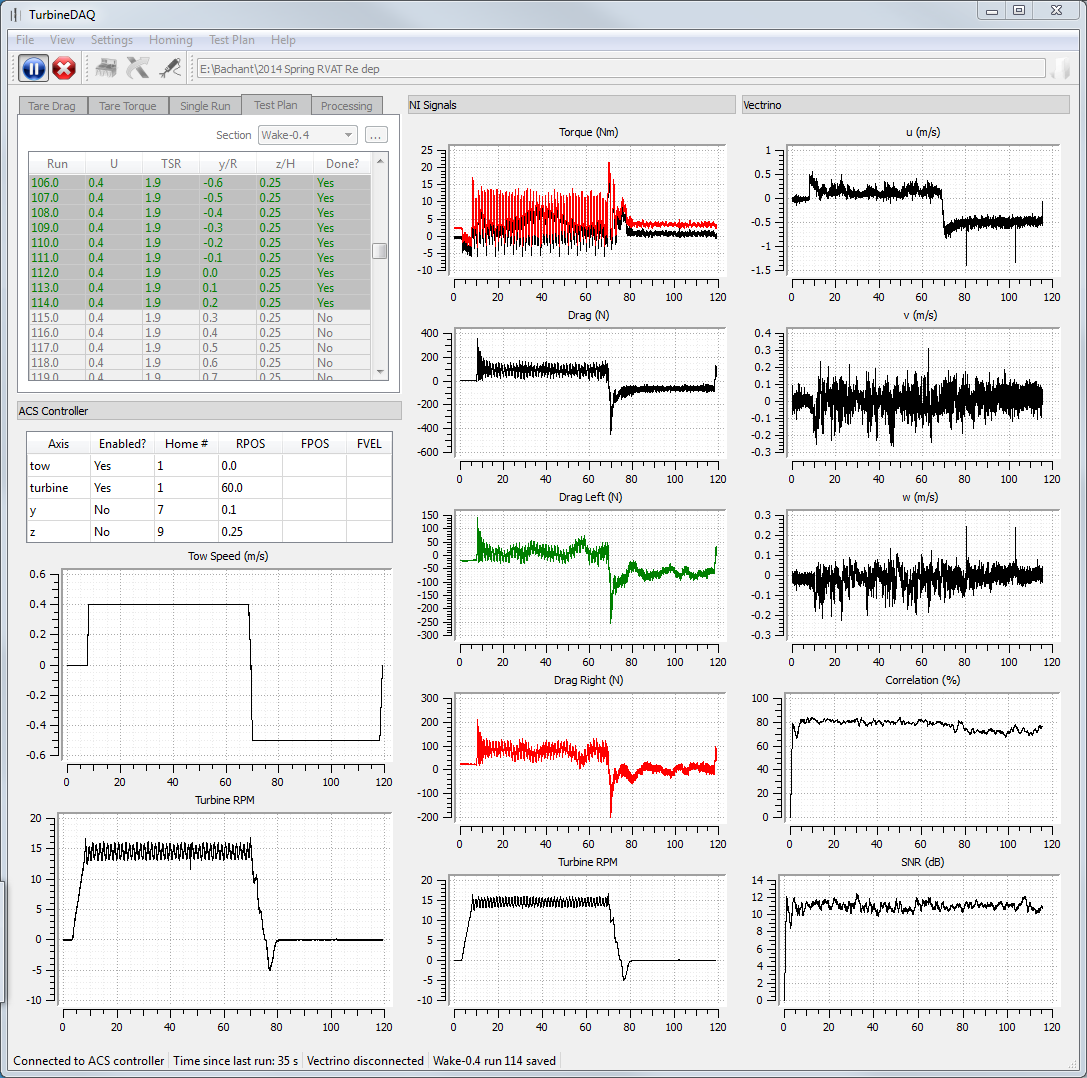
\includegraphics[width=0.9\textwidth]{Figures/TurbineDAQ}
\caption{Screenshot from the \textit{TurbineDAQ} experiment automation software,
developed for vertical-axis turbine measurements in the UNH tow tank.}
\label{fig-turbinedaq}
\end{figure}


\begin{figure}
\begin{verbatim}
RM2-tow-tank/
    Config/
        Test plan/
            perf_0.8.csv
            wake_0.25.csv
            tare_drag.csv
            tare_torque.csv
            settling.csv
            perf_strut_drag.csv
            stat_strut_torque.csv
        turbine_properties.json
        settling_times.csv
        raw_data_urls.json
    Data/
        Processed/
            perf_0.8.csv
        Raw/
            perf_0.8/
                0/
                    metadata.json
                    acsdata.h5
                    nidata.h5
                    vecdata.h5
                    vecdata.vno
                1/    
                    metadata.json
                    acsdata.h5
                    nidata.h5
                    vecdata.h5
                    vecdata.vno
    Documents/
        Test plan/
        Final report/
    Scripts/
    README.md
\end{verbatim}
\caption{Sample directory structure for experiment configuration, data, and
documentation.} \label{fig-dir_structure}
\end{figure}

\begin{table}[ht]
\centering
\begin{tabular}{l|l|l|l}
Data & Sample rate & File type & File name \\
\hline 
\begin{tabular}[t]{@{}l@{}}
\texttt{time} \\
\texttt{carriage\_pos} \\
\texttt{turbine\_angle} \\
\texttt{torque\_trans} \\
\texttt{torque\_arm} \\
\texttt{drag\_left} \\
\texttt{drag\_right}
\end{tabular} & 2 kHz & HDF5 & \texttt{nidata.h5} \\ 
\hline
\begin{tabular}[t]{@{}l@{}}
\texttt{time} \\
\texttt{carriage\_vel} \\
\texttt{turbine\_rpm} \\
\end{tabular} & 1 kHz & HDF5 & \texttt{acsdata.h5} \\ 
\hline
\begin{tabular}[t]{@{}l@{}}
\texttt{time} \\
\texttt{u} \\
\texttt{v} \\
\texttt{w} \\
\texttt{corr\_u} \\
\texttt{corr\_v} \\
\texttt{corr\_w} \\
\texttt{snr\_u} \\
\texttt{snr\_v} \\
\texttt{snr\_w}
\end{tabular} & 200 Hz & HDF5 & \texttt{vecdata.h5} \\ 
\hline
\begin{tabular}[t]{@{}l@{}}
\texttt{vecdata.dat} \\
\texttt{vecdata.hdr} \\
\texttt{vecdata.pck} \\
\end{tabular} & 200 Hz & Vectrino binary & \texttt{vecdata.vno} \\ 

\end{tabular}
\caption{Raw data file description.}
\label{tab-data_description}
\end{table}

\end{appendices}

\end{document}